\chapter{Implementation}
\label{chapter5}


In section, we will explain the implement of the seq2seq model with LSTM, which has been described in Section~\ref{chapter3} and Section~\ref{chapter4} in detail. Besides the implementation, the method of processing and generating the training and testing dataset will also be introduced in this section. Then, we will train a neural network model by using the generated training dataset and evaluate the trained network model by the generated testing dataset. In a word, we will describe the dataset, implementation, training and evaluation in the following.

\section{Dataset}
Building error correction systems by applying the machine learning techniques usually needs a large amount of annotated data, which is difficult to obtain. In addition, the available error-annotated corpora are often focused on specific groups of people (e.g. non-native students), error types (e.g. spelling, syntax), genres (e.g. university essays, letters) or topics. Consequently, we cannot grantee that these datasets is representative enough for training the models and or the trained GEC system is general enough in different scenarios. On the other hand, building new corpora is not always a viable solution since error annotation by human is expensive. Focusing on the existing dataset, the grammatical error correction has various datasets such as Conll and JFLEG \cite{ng2014conll,napoles2017jfleg}. However, these datasets are usually used as a testing set to check if the proposed algorithm perform well and the dataset is relatively small for training. Thus, building a proper dataset for training our model is the first thing we need to focus on.

\cite{felice2014generating} show that it is possible to generate artificial grammatical errors to build up a training dataset for the grammatical error correction. They also show that using carefully generated artificial errors can even improve the performance of error correction systems. Felice’s work brings us a good new for GEC training dataset building.

To create a dataset for training and evaluation, we need to start with a large collection of mostly grammatically correct samples of conversational written valuation English. The primary dataset considered in this project is the Cornell Movie-Dialogs Corpus (CMDC). The CMDC has over 300k lines from movie scripts. This is the largest collection of conversational written English we can grantee grammars in which are mostly correct.

After getting the CMDC data, the next step we need is to generate input-output pairs. These pairs will be used for training GEC system. The error generation for the input-output pairs can be done in the following steps:

\begin{itemize}
    \item Read each line from the CMDC file. The format of CMDC dataset is that each line of the file is a sentence.
    \item Randomly choose one kind of grammatical errors and apply the corresponding error generation on the current read sentence, which is called random perturbations. The distribution of each grammatical error is as the same grammatical error distribution of the famous dataset CoNLL 2014.
    \item Pair the unperturbed sentence and perturbed sentence. Write the train pair into the training dataset file.
\end{itemize}
where the perturbations applied in step (2) are intended to introduce small grammatical errors which we would like the model to learn to correct. Thus far, these perturbations of grammatical errors are limited to:
\begin{itemize}
    \item Subtraction of articles (a, an, the)
    \item Subtraction of the second part of a verb contraction (e.g. “ve”, “ll”, “s”, “m”)
    \item Replacement of a few common homophones with one of their counterparts (e.g. replacing "their" with "there", "then" with "than")
\end{itemize}
The rates of these perturbation types are introduced are loosely based on figures taken from the CoNLL 2014 Shared Task on Grammatical Error Correction \cite{ng2014conll}. In this project, each perturbation is applied in $25\%$ of cases where it could potentially be applied.
\begin{figure}[ht]
    \centering
    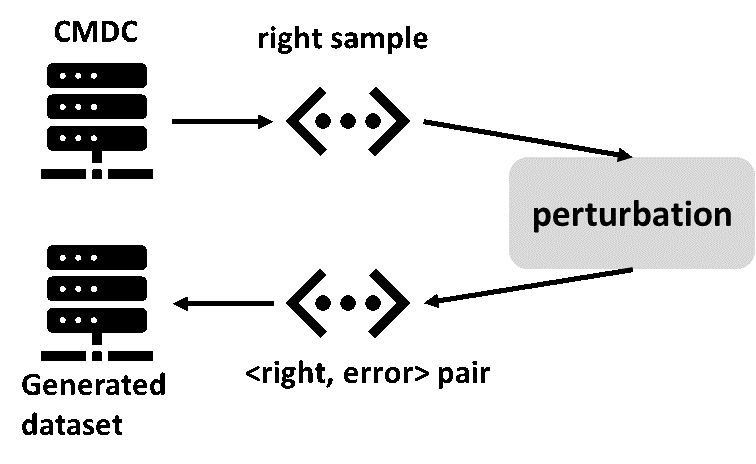
\includegraphics[width=0.8\textwidth]{AEGD.png}
    \caption{Artifical error generation for Dataset.}
    \label{fig:8}
\end{figure}

\section{Implementation}
To artificially increase the dataset amount when training the built seq2seq model, we apply the sampling strategy described above multiple times to arrive at 2-3 times of the number of input-output pairs. Given this augmented dataset, training can be executed in a similar manner to seq2seq model training of the previous existing works. That is, we train a sequence-to-sequence model using LSTM encoders and decoders with an attention mechanism as described in \cite{bahdanau2014neural} using stochastic gradient descent.

\subsection{Decoding}

Instead of using the most probable decoding according to the seq2seq model, this project takes advantage of the unique structure of this problem to impose the prior that all tokens in a decoded sequence should either exist in the input sequence or belong to a set of "corrective" tokens. The "corrective" token set is constructed during training and contains all tokens seen in the target, but not the source, for at least one sample in the training set. The intuition here is that the errors which are marked during training involve the misuse of a relatively small vocabulary of common words (e.g. "the", "an", "their") and that the model should only be allowed to perform corrections in this domain.

This prior is carried out through a modification to the seq2seq model's decoding loop in addition to a post-processing step that resolves out-of-vocabulary (OOV) tokens:

\begin{itemize}
    \item Biased Decoding: This project applies a binary mask to the model's logits prior to extracting the prediction to be fed into the next time step. This can restrict the decoding such that it only ever chooses tokens from the input sequence or corrective token set. The mask is constructed in the following way
    \begin{align}
    Mask[i]=
    \begin{cases}
        1, i \; in \; input\; or\; corrective\_tokens\\
        0, else
    \end{cases}
    \end{align}
    Since this mask is applied to the result of a softmax transformation. This transformation can guarantees all outputs are non-negative. We can be sure that only input or corrective tokens are ever selected. Note that this logic is not used during training, as this would only serve to eliminate potentially useful signal from the model.
    \item Handling OOV Tokens: Since the decoding bias described above is applied within the truncated vocabulary used by the model, we will still see the unknown token in its output for any OOV tokens. The more generic problem of resolving these OOV tokens is non-trivial (e.g. see Addressing the Rare Word Problem in NMT), but in this project we can again take advantage of its unique structure to create a straightforward OOV token resolution scheme. That is, if we assume the sequence of OOV tokens in the input is equal to the sequence of OOV tokens in the output sequence, then we can trivially assign the appropriate token to each "unknown" token encountered in the decoding. Empirically, and intuitively, this appears to be an appropriate assumption, as the relatively simple class of errors these models are being trained to address should never include mistakes that warrant the insertion or removal of a rare token.
\end{itemize}

\subsection{Details}
This project reuses and slightly extends TensorFlow's Seq2SeqModel, which itself implements a sequence-to-sequence model with an attention mechanism as described in tensorflow’s tutorial document. The primary function file we use is described as the following:
\begin{itemize}
    \item \texttt{data\_reader.py}: an abstract class that defines the interface for classes which can read a source dataset and producing input-output pairs, where the input is a grammatically incorrect variant of a source sentence and the output is the original sentence.
    \item \texttt{text\_corrector\_data\_readers.py}: contains a few implementations of DataReader which is over the CMDC.
    \item \texttt{text\_corrector\_models.py}: contains a version of Seq2SeqModel modified such that it implements the logic described in Biased Decoding.
    \item \texttt{correct\_text.py}: a collection of helper functions that together allow for the training of a model and the usage of it to decode errant input sequences (at test time). The decode method defined here implements the OOV token resolution logic. This also defines a main method and can be invoked from the command line. It was largely derived from TensorFlow's translate.py.
\end{itemize}

